% Created 2022-04-14 Thu 13:43
% Intended LaTeX compiler: pdflatex
\documentclass[presentation]{beamer}
\usepackage[utf8]{inputenc}
\usepackage[T1]{fontenc}
\usepackage{graphicx}
\usepackage{grffile}
\usepackage{longtable}
\usepackage{wrapfig}
\usepackage{rotating}
\usepackage[normalem]{ulem}
\usepackage{amsmath}
\usepackage{textcomp}
\usepackage{amssymb}
\usepackage{capt-of}
\usepackage{hyperref}
\hypersetup{colorlinks=true,linkcolor=blue}
\usetheme{Madrid}
\author{Cody Harris}
\date{\textit{<2022-04-14 Thu>}}
\title{Ultrafast userspace packet blasting: Why should the kernel have all the fun?}
\hypersetup{
 pdfauthor={Cody Harris},
 pdftitle={Ultrafast userspace packet blasting: Why should the kernel have all the fun?},
 pdfkeywords={},
 pdfsubject={What is graph reduction? Why should you care?},
 pdfcreator={Emacs 27.1 (Org mode 9.4.5)},
 pdflang={English}}
\begin{document}

\maketitle
\begin{frame}{Outline}
\tableofcontents
\end{frame}


\section{Network Programming, the Usual Way}
\label{sec:orgb6d1f38}

\section{Network Programming, the Unusual Way (in userspace)}
\label{sec:org84fcd63}
\begin{frame}[label={sec:org375ef4f}]{But Why?}
\begin{itemize}
\item Writing kernel code is really hard.
\begin{itemize}
\item Small mistakes crash the whole system.
\item Libraries are different, less featured.
\end{itemize}
\item Debugging kernel code is even harder than writing it.
\item Userspace code is just as fast as the kernel on a properly-configured system.
\begin{itemize}
\item Actualy, userspace code can be even faster than the kernel --it can focus on just one thing.
\end{itemize}
\end{itemize}
\end{frame}
\begin{frame}[label={sec:org74ee6b4}]{What's Wrong with the Kernel Network Stack?}
\begin{itemize}
\item Nothing is wrong with the kernel network stack, but sometimes you
run up against its limits.
\begin{itemize}
\item Want to do weird things it wasn't meant to do
\item Need higher performance than it was designed to provide (eg.
use a commodity server as a network device)
\item The kernel network stack is mostly interrupt-driven
\begin{itemize}
\item A reasonable choice for a general-purpose system!
\item But interrupt-driven is a compromise when net throughput is
highest priority
\item Polling (repeatedly checking) network card is faster than
waiting to be told that packets have arrived
\end{itemize}
\end{itemize}
\end{itemize}
\end{frame}
\begin{frame}[label={sec:org1f777c2}]{But How? (Applies to any High-Performance System)}
\begin{itemize}
\item Configure the system for high performance.
\begin{itemize}
\item Disable features that throttle back the CPU clock
\item Configure huge pages to improve memory performance
\item Disable SMI interrupts from the BIOS
\end{itemize}
\item Configure the kernel so it's out of the way
\begin{itemize}
\item Pin your processes to specific cores
\item Configure the kernel to never schedule other processes (inc.
itself) on your cores (via isolcpus)
\item Go tickless, disable RCU callbacks so the kernel doesn't interrupt
\item You now have the whole core to yourself!
\end{itemize}
\item Don't use system calls in high-performance code
\begin{itemize}
\item Just use counters, no logging in normal operation
\item Ok, major errors and RPC can go to a shared-memory ring-buffer,
but NO printf allowed!
\end{itemize}
\end{itemize}
\end{frame}
\begin{frame}[label={sec:org6ac71fd}]{But How? (Network Specifics)}
\begin{itemize}
\item Get the kernel network stack out of the way
\item Unbind the network card from the kernel network driver
\item Bind the network card to a userspace i/o driver
\begin{itemize}
\item This memory-maps the network card's address space into
userspace. You can talk to the card just by reading and writing
to memory. PCIe subsystem handles the bus transparently. Feels
like embedded system programming.
\end{itemize}
\item Use a userspace driver (just some C code) to talk to the network
card with a nicer API
\item One downside --you no longer have a network stack
\end{itemize}
\end{frame}
\begin{frame}[label={sec:orgd96bbfc}]{But How? (Network Card Specifics)}
\begin{itemize}
\item Configure network card checksum offloads to save some work
\begin{itemize}
\item Cards have logic to verify or generate:
\begin{itemize}
\item Ethernet frame CRC
\item IP header checksum
\item UDP or TCP checksums
\end{itemize}
\end{itemize}
\item Split the network card into multiple queues
\begin{itemize}
\item A modern high-performance server CPU can only forward about 1
Gbps of traffic per core.
\item Eg. make your 10GbE card act like 20x 0.5 Gbps pipes.
\begin{itemize}
\item Gives you headroom to actually do something with the packets!
\end{itemize}
\end{itemize}
\item Set up memory for the network card
\begin{itemize}
\item Message buffers --where packet data goes
\item Descriptors --a card-specific data structure understood by the
network card. One descriptor per packet. These describe the DMA
setup and tells the network card where the message buffers are.
\item Descriptors are in a ring buffer (a linked list where the tail
points back to the head)
\end{itemize}
\end{itemize}
\end{frame}
\begin{frame}[label={sec:org7c44d43}]{The Data Plane Development Kit (DPDK)}
\begin{itemize}
\item Open source project started by Intel
\item Provides libraries to handle the really tedious parts of
everything just mentioned
\item A hardware abstraction layer and the userspace network card
drivers.
\begin{itemize}
\item They've implemented userspace poll-mode drivers (PMDs) for
popular network cards
\begin{itemize}
\item (In contrast to more common interrupt-driven drivers)
\end{itemize}
\end{itemize}
\item Contains useful lockless data structures
\end{itemize}
\end{frame}

\begin{frame}[label={sec:org5621daa}]{No Gods No Masters}
\begin{itemize}
\item You are no longer bound by the rules of society
\item Any frame/packet headers you want, including addresses:
\begin{center}
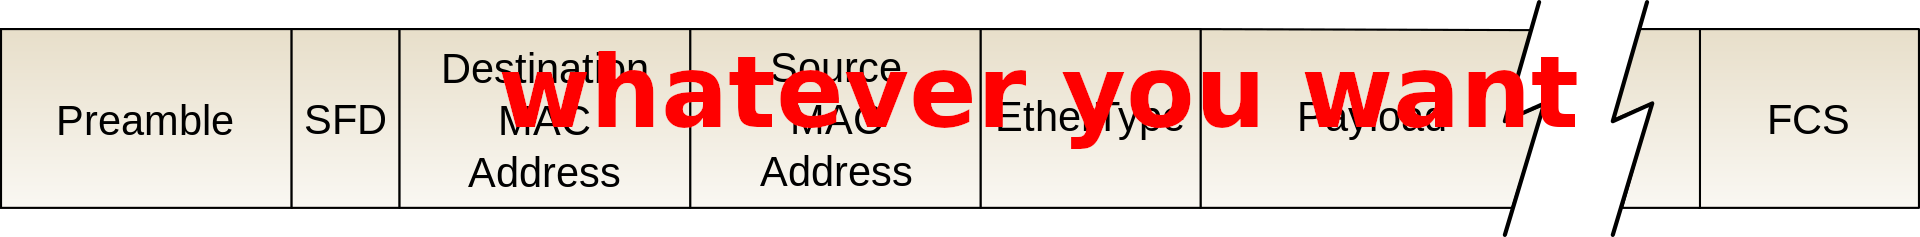
\includegraphics[width=1.0\linewidth]{./ethernet.png}
\end{center}
\begin{itemize}
\item Any ethernet src/dst (pretend to be many computers for the lulz)
\item Anything layer-3 payload want inside the ethernet frame. IP is
nice if you want your packets to get onto the internet, but
there are many interesting layer-3 protocols:
\url{https://en.wikipedia.org/wiki/EtherType} has some interesting
ideas for protocols to implement:
\begin{itemize}
\item GOOSE, SVE, GSE --SCADA and industrial control!
\item IPX, DECnet --Network with vintage computers, bridge them to
the internet?
\item Precision Time Protocol (PTP) client or server?
\end{itemize}
\end{itemize}
\end{itemize}
\end{frame}

\begin{frame}[label={sec:orgbaff8b2}]{No Gods No Masters (Continued)}
\begin{itemize}
\item Make IP packets, send them to the internet\ldots{}
\begin{itemize}
\item Fake the source address, see what happens
\item Ping everybody on the internet: \(\frac{3.7 \cdot 10^9 \text{addresses}}{1.49 \cdot 10^6 \text{packets/second}}\)
\begin{itemize}
\item 2500 seconds to ping every public ip4 address with a 1 Gbps link!
\end{itemize}
\item Implement a scary fast port scanner?
\end{itemize}
\end{itemize}
\end{frame}

\begin{frame}[label={sec:org4b2ed3c}]{Slightly More Practical Ideas}
\begin{itemize}
\item Implement NAT (network address translation) to bridge networks.
\item Network wiretap and deep-packet inspection device that mirrors
packet off to some secret cable :nsa:
\item Implement a high-performance network tunnel endpoint, eg. IPSec
VPN
\begin{itemize}
\item Network virtualization! Become your own cloud provider!
\end{itemize}
\item Build a firewall, switch, router, etc. in software
\end{itemize}
\end{frame}

\section{DPDK Setup}
\label{sec:org6a198c2}
\begin{frame}[label={sec:org5a66088}]{Download and install DPDK}
\begin{itemize}
\item Get it from dpdk.org
\item My opinion: work from a release tag, not HEAD, for the best experience
\end{itemize}
\end{frame}

\begin{frame}[label={sec:org61cef06}]{Configure machine for hugepages}
\begin{block}{What is a page?}
\begin{itemize}
\item Basically a chunk of RAM. 4KB in modern Linux machines.
\item Why divide memory up into pages? Virtual memory. Outside scope of this talk, but a fascinating topic.
\end{itemize}
\end{block}
\begin{block}{What are hugepages?}
\begin{itemize}
\item Like pages, but huger. 2MB or 1GB chunks (configurable) rather than 4KB.
\item Why would I do use hugepages? Hardware reasons. Sort-of out of scope.
\end{itemize}
\end{block}
\end{frame}
\begin{frame}[label={sec:orgc11a540}]{But Hardware is Cool, so if there's Time:}
\begin{itemize}
\item The translation lookaside buffer (TLB) is a hardware component in
the CPU's virtual memory system.
\item TLB speeds up virtual memory via table of mappings between virtual addresses and physical addresses.
\begin{itemize}
\item Pages cached in the TLB can be accessed immediately.
\item Pages that aren't in the TLB can still be accessed, but there's
a performance impact because the kernel needs to step in and
help (context switch).
\end{itemize}
\item This all happens transparently to a userspace program, but there
is a performance impact to TLB misses.
\item Bigger pages -> fewer pages. fewer pages -> fewer opportunities
for tlb misses. tlb miss requires context switch to kernel, which
is slow. Default pages are 4KB. Huge pages are 2MB or 1GB on
modern CPUs
\end{itemize}
\end{frame}
\begin{frame}[label={sec:orge842218},fragile]{Configuring Hugepages}
 \begin{itemize}
\item First, requires build-time support from kernel
\item I had to edit /etc/sysctl.conf and add vm.nr\textsubscript{hugepages} = \ldots{} (set a different option if you want to use 1G hugepages) then reboot
\item You can check for success in /proc/meminfo
\begin{verbatim}
# grep Huge /proc/meminfo
AnonHugePages:         0 kB
ShmemHugePages:        0 kB
FileHugePages:         0 kB
HugePages_Total:     256
HugePages_Free:      245
HugePages_Rsvd:      125
HugePages_Surp:        0
Hugepagesize:       2048 kB
Hugetlb:          524288 kB
\end{verbatim}
\end{itemize}
\end{frame}

\begin{frame}[label={sec:org6eb6044}]{Bind network card to a vfio driver}
\begin{itemize}
\item What? The network card "owns" a section of memory. In non-DPDK
world, the kernel driver reads and writes this memory to make it
do network things. In DPDK world, we need to read/write this
memory from userspace. Basically, the vfio driver mmaps the
network card so we can mess with the hardware directly from
userspace.
\end{itemize}
\end{frame}

\begin{frame}[label={sec:org956b3a3},fragile]{How To Do It}
 \begin{verbatim}
# sudo modprobe uio_pci_generic # load userspace PCI driver
# ./usertools/dpdk-devbind.py -s # list the current bindings
Network devices using kernel driver
===================================
0000:00:1f.6 [...] drv=e1000e unused=uio_pci_generic

# ./usertools/dpdk-devbind.py -u 00:1f.6 # unbind NIC driver

# bind uio to ethernet NIC instead of kernel network driver
# ./usertools/dpdk-devbind.py -b uio_pci_generic 00:1f.6

#./usertools/dpdk-devbind.py -s # list bindings again
Network devices using DPDK-compatible driver
============================================
0000:00:1f.6 [...] drv=uio_pci_generic # woohoo
\end{verbatim}
\end{frame}
\end{document}
